% !TEX root = BachelorBookletMain.tex

\chapter{Maze Game Systems}\label{MazeGameSystems}
 In this Prototype the player has to navigate though a maze. He has to use the network output to navigate. There are several enemy types that have to be avoided or destroyed. Multiple objects have to be collected before the exit is unlocked.

\section{Audio}
In this project I use the Resonance Audio plug-in to simulate spacial sound. This facilitates player orientation. All important objects and events such as enemies and checkpoints emit a unique sound, that helps to spatially locate and identify them. A doppler effect is used on all audiosources, so the player perceives how entities are moving relative to him.


\section{Sound spectrum analyzing materials}
I created a simple sound spectrum analyzing script, that when attached to an object automatically varies the intensity of the objects material color based on the current spectrum of the objects audio source. Parameters are exposed to define ranges for valid color intensities and to set how the spectrum should be filtered before its intensity is determined.


\section{Checkpoints}
To beat a level the player has to collect all checkpoints. They are visualized as green rectangular cuboids that vary their material using the spectrum analyzing script (\cref{SonarBlinks}). Periodically a checkpoint emits a high pitched, slowly decaying ping sound. Because the sound is specialized with Resonance Audio, the player can use this audio signal to determine the direction and distance to the checkpoint. Only one checkpoint is active at a time, and a new checkpoint only activates if the current one has been collected. This makes it easier for the player to home in on the sound. The final checkpoint, refereed to as goal, has the same audio signal but different visuals (\cref{GoalBlinks}) and triggers the game won state when reached.

\begin{figure}[p]
  \centering
  
\includegraphics[width=\imgWidth]{images/game_systems/CheckpointDim.png} \\[\picVdist]
  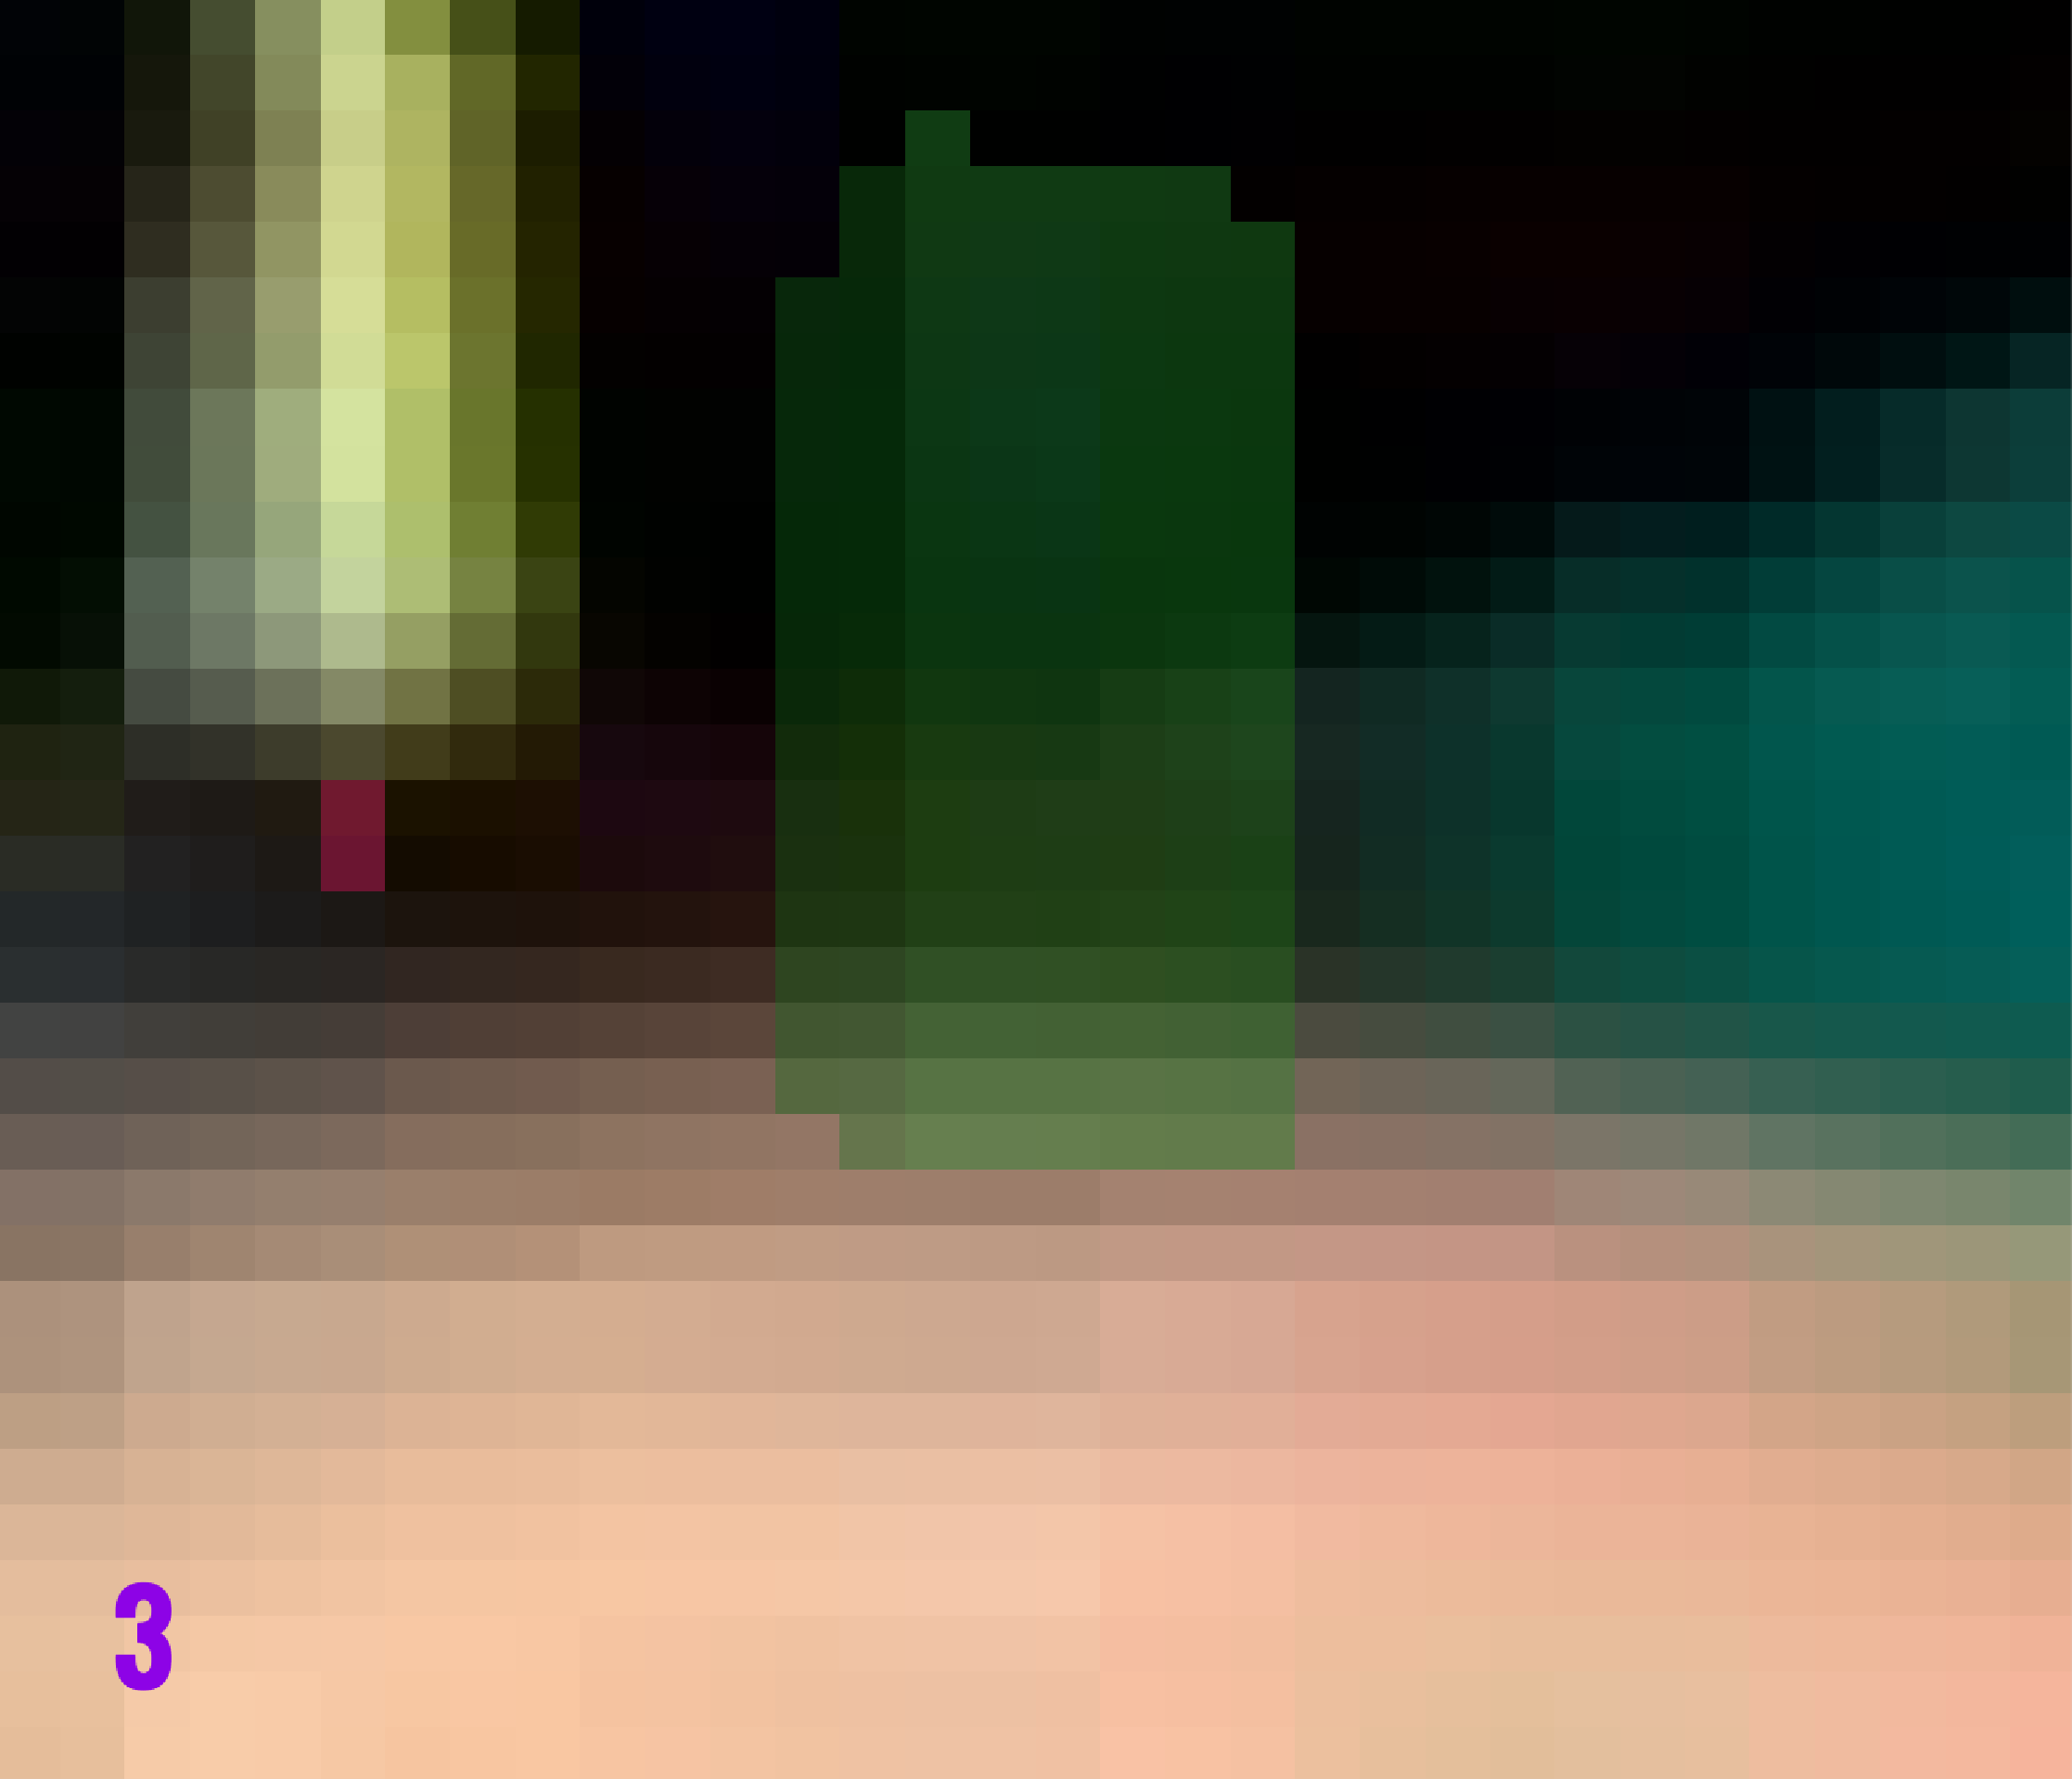
\includegraphics[width=\imgWidth]{images/game_systems/CheckpointBright.png}
  \caption{Checkpoint cuboid varying material color based on the current sound}
  \label{SonarBlinks}
  \figsource{own graphic}
\end{figure}

\begin{figure}[p]
  \centering
  
\includegraphics[width=\imgWidth]{images/game_systems/GoalDim.png} \\[\picVdist]
  
\includegraphics[width=\imgWidth]{images/game_systems/GoalBright.png}
  \caption{Checkpoint cuboid varying material color based on the current sound}
  \label{GoalBlinks}
  \figsource{own graphic}
\end{figure}


\section{Enemies}
Enemies in this prototype all follow a simple pattern. They spawn out of a for the player visible spawn point and move in a straight line across the map. How they move is different for each enemy type. Each of them emits a sound that helps to identifies them. They are all pyramid shaped with the apex pointing in the flight direction, to give them the association that they are dangerous.


\subsection{Speeder}
\Cref{Speeder} shows the simplest enemy, the speeder. He moves forward with a constant velocity. This enemy emits a two sounds. One can only be heard by the player if the enemy is moving directly at him. A variation of the speeder exists that moves way faster and looks different (\cref{FastSpeeder}). Because of the doppler effect applied to the audio sources the sound emmitted feels more dangerous. This is probably because with the doppler sound you also hear that it goes really fast.

\begin{figure}[p]
  \centering
  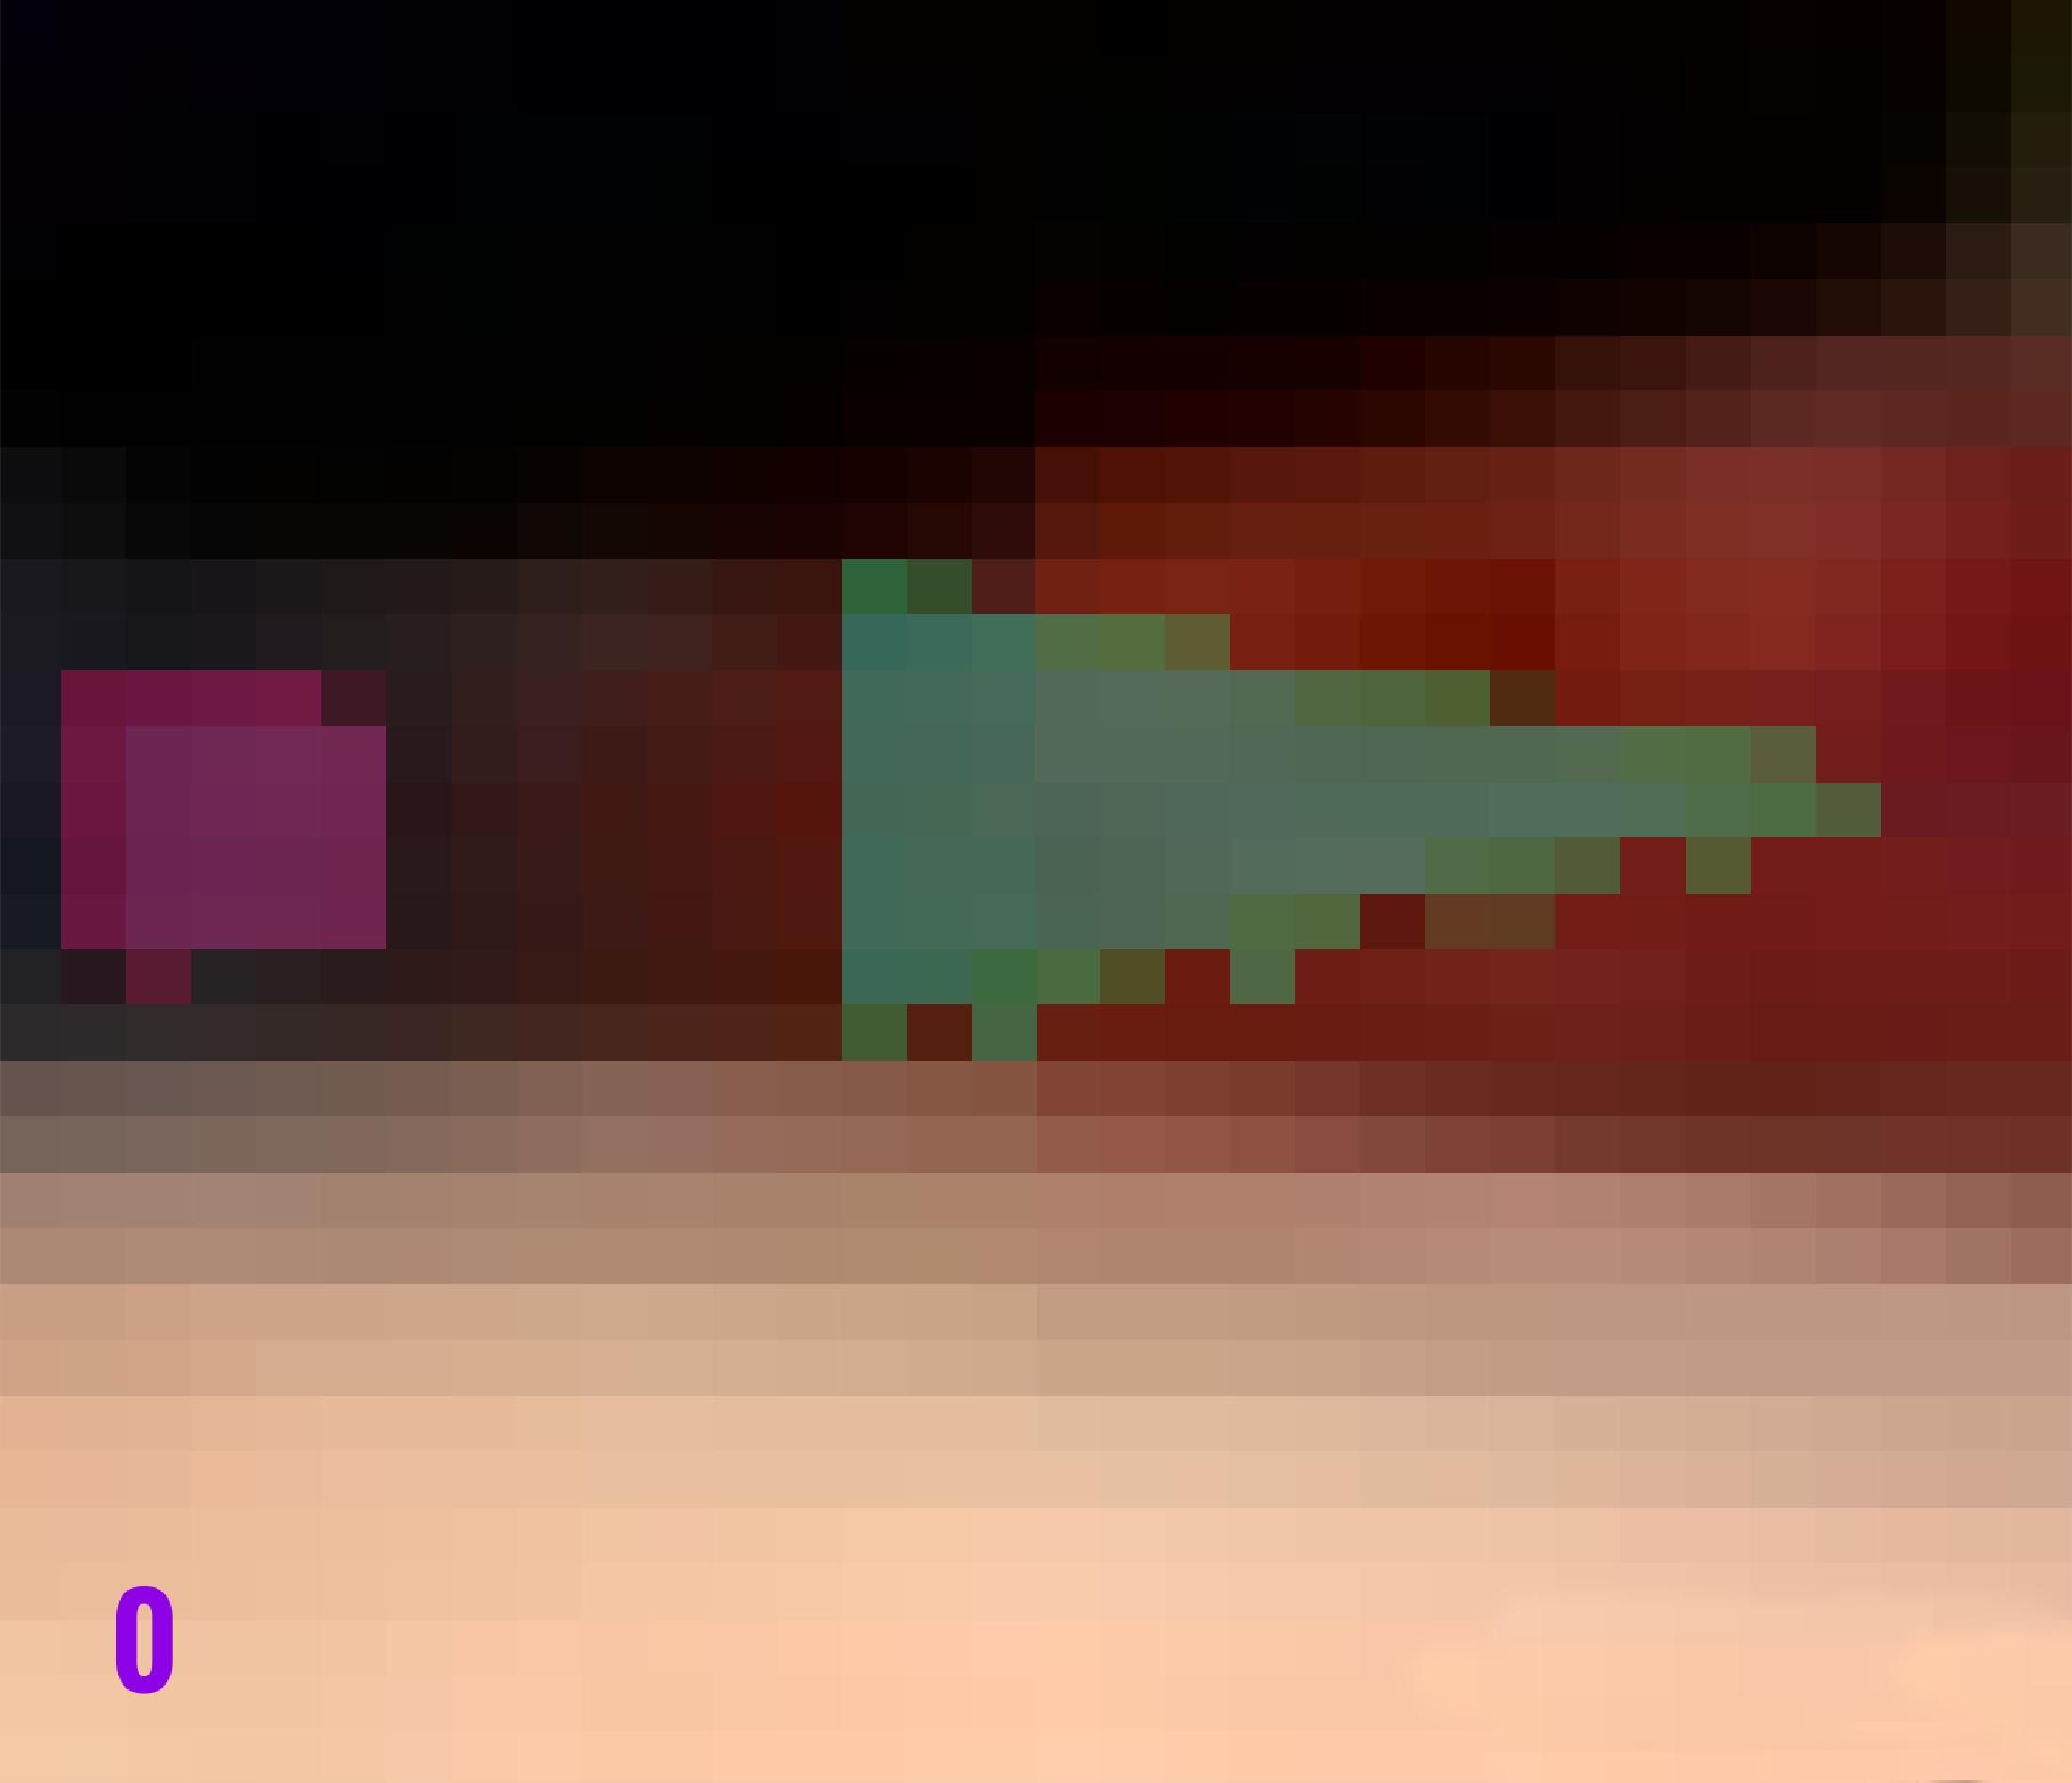
\includegraphics[width=\imgWidth]{images/game_systems/SpeederSpawns.png}
  \caption{Speder moves away from his pink spawn point}
  \label{Speeder}
  \figsource{own graphic}
\end{figure}

\begin{figure}[p]
  \centering
  
\includegraphics[width=\imgWidth]{images/game_systems/FastSpeeder.png}
  \caption{A variation of the speeder that moves faster}
  \label{FastSpeeder}
  \figsource{own graphic}
\end{figure}


\subsection{Invisible champer}\label{InvisibleChamper}
This enemy moves just like the speeder. However the champer is a much harder enemy because he is invisible most of the time. Periodically he makes a champing sound. Using the spectrum analyzing script the material is adjusted to make the champer visible for a brief period every time he emits a sound (\cref{Champer}).

\begin{figure}[p]
  \centering
  
\includegraphics[width=\imgWidth]{images/game_systems/ChamperInvisible.png} \\[\picVdist]
  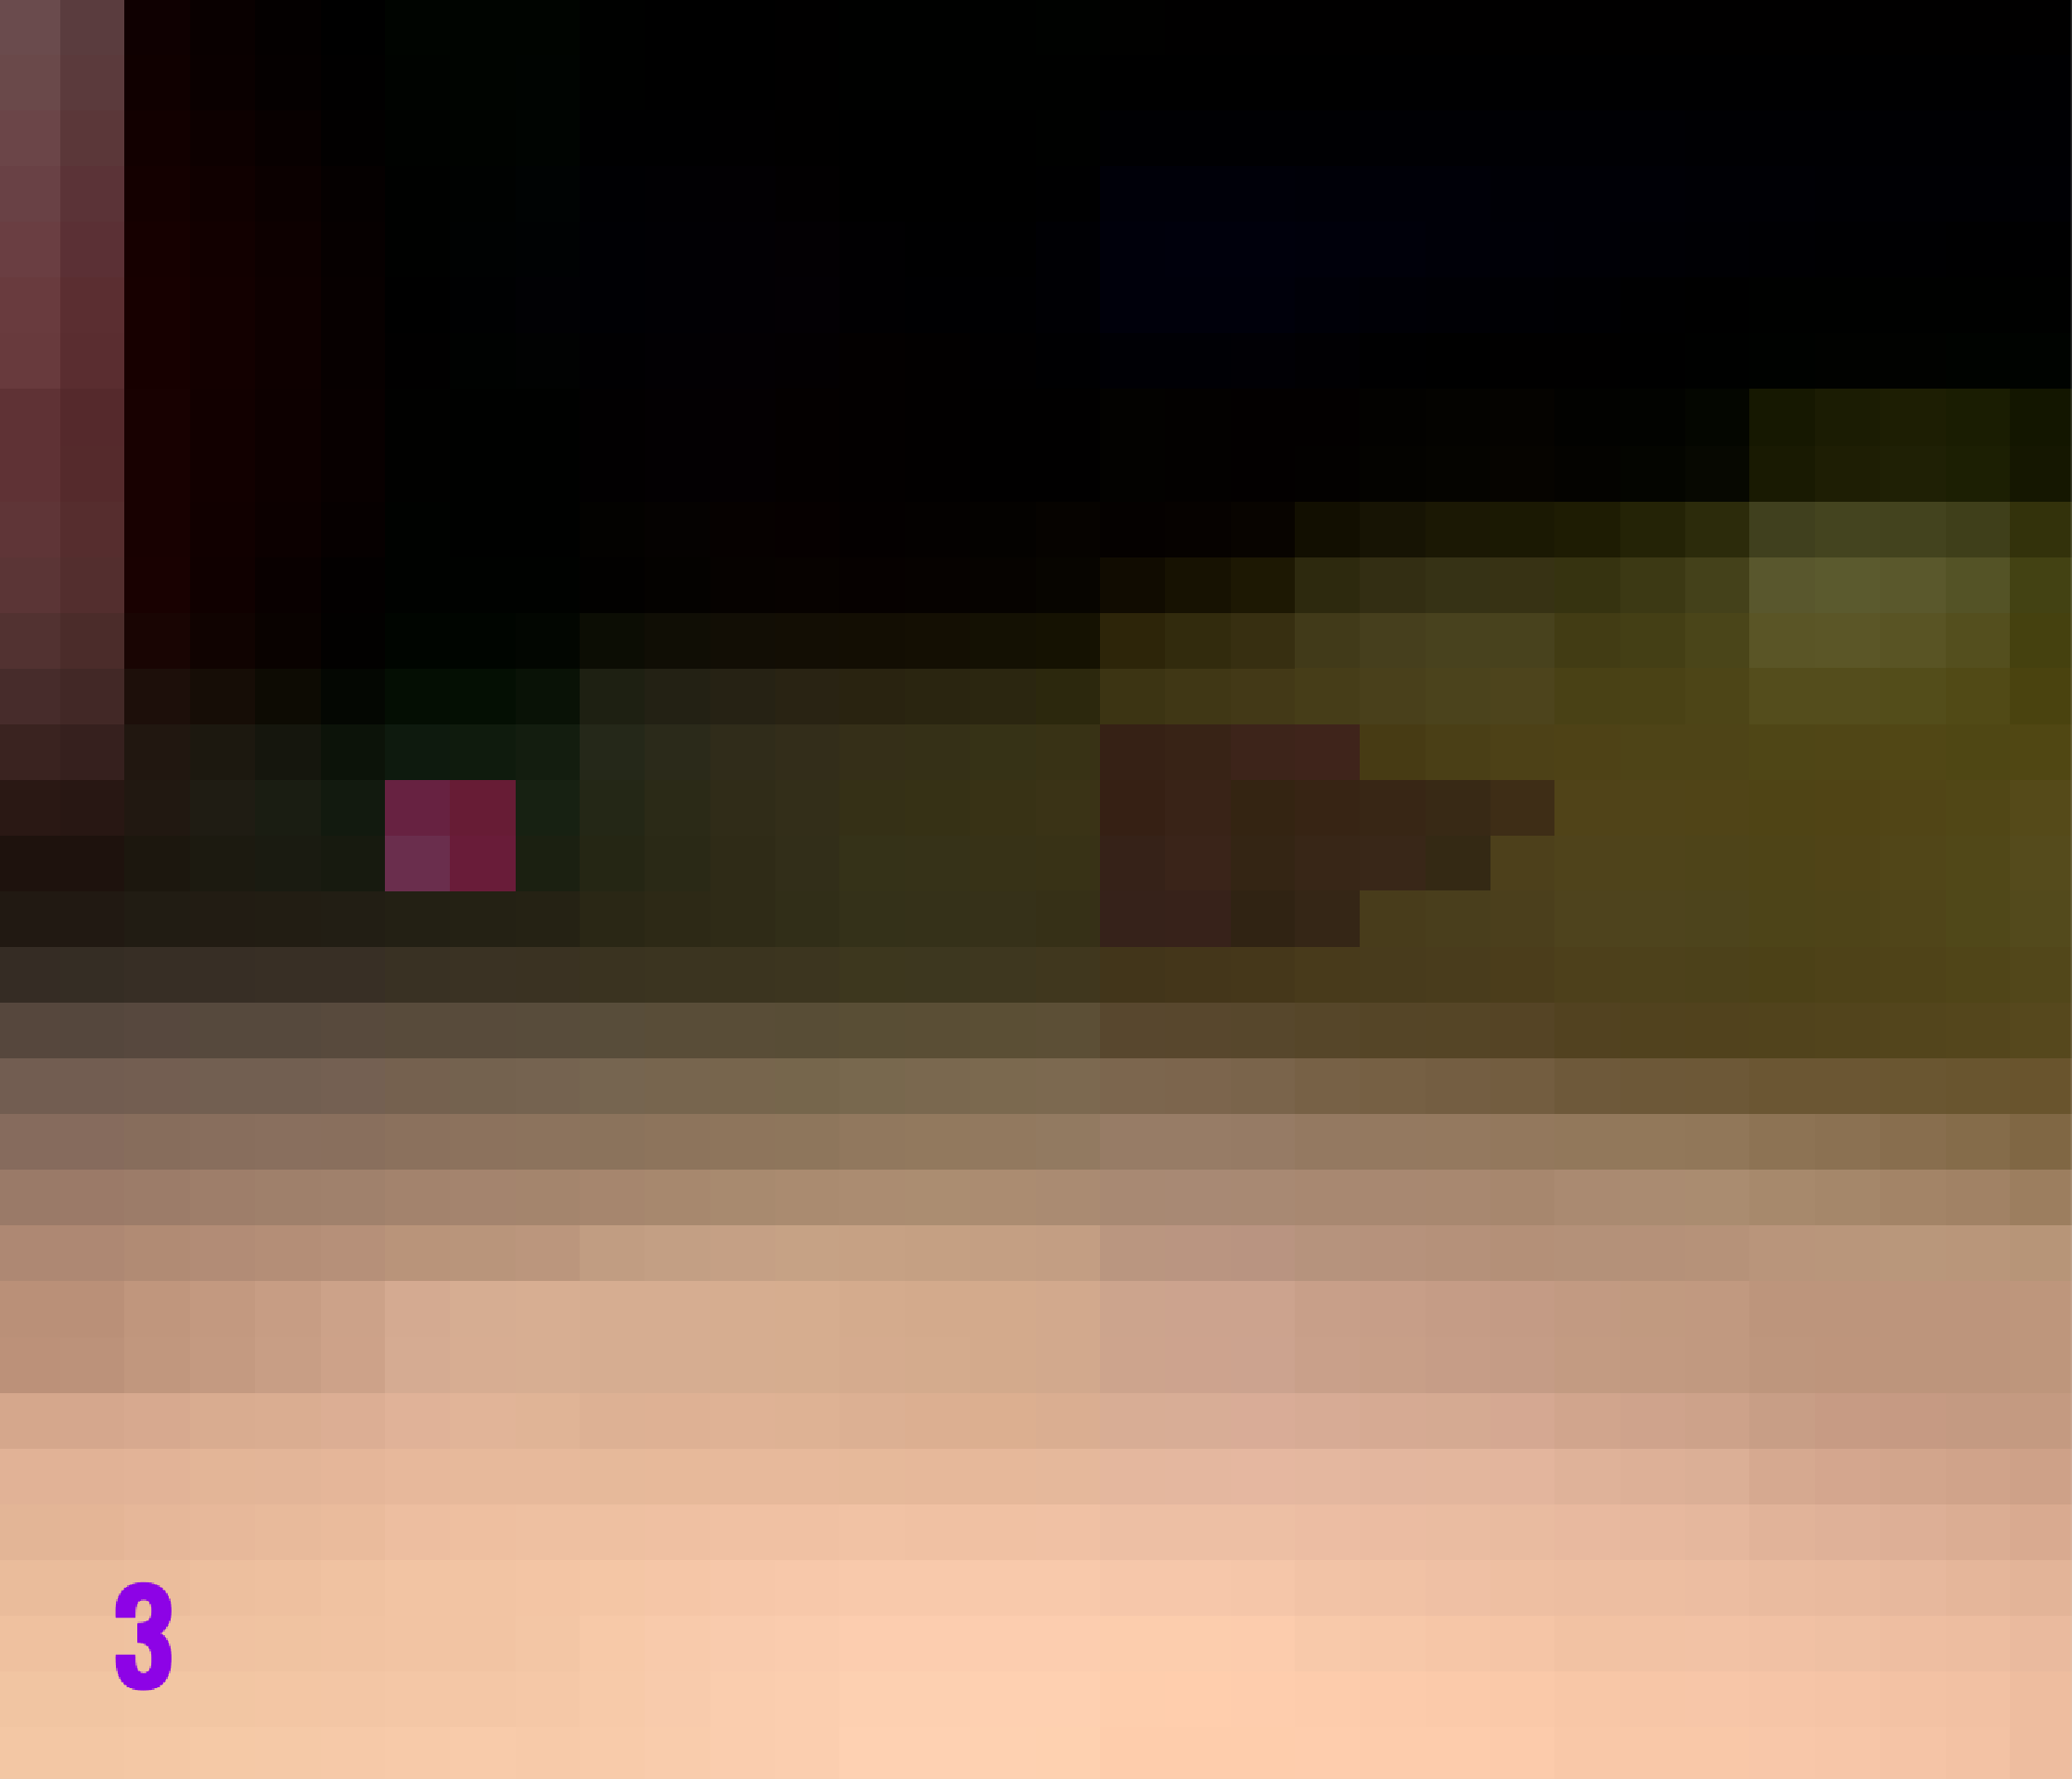
\includegraphics[width=\imgWidth]{images/game_systems/ChamperVisible.png}
  \caption{A champer becomes visible because he emits a sound}
  \label{Champer}
  \figsource{own graphic}
\end{figure}


\subsection{DumDum}
The DumDum uses a script that analyzes the sound spectrum of the attached audio source to determine his movement speed. The audio source loop of the DumDum consists of four short pulses of sound and a long pause. Each time one of the pulses is played the DumDum starts to move until the pulse stops. This leads to the DumDum rapidly jumping forward four times before becoming stationary for brief period of time.

\begin{figure}[p]
  \centering
  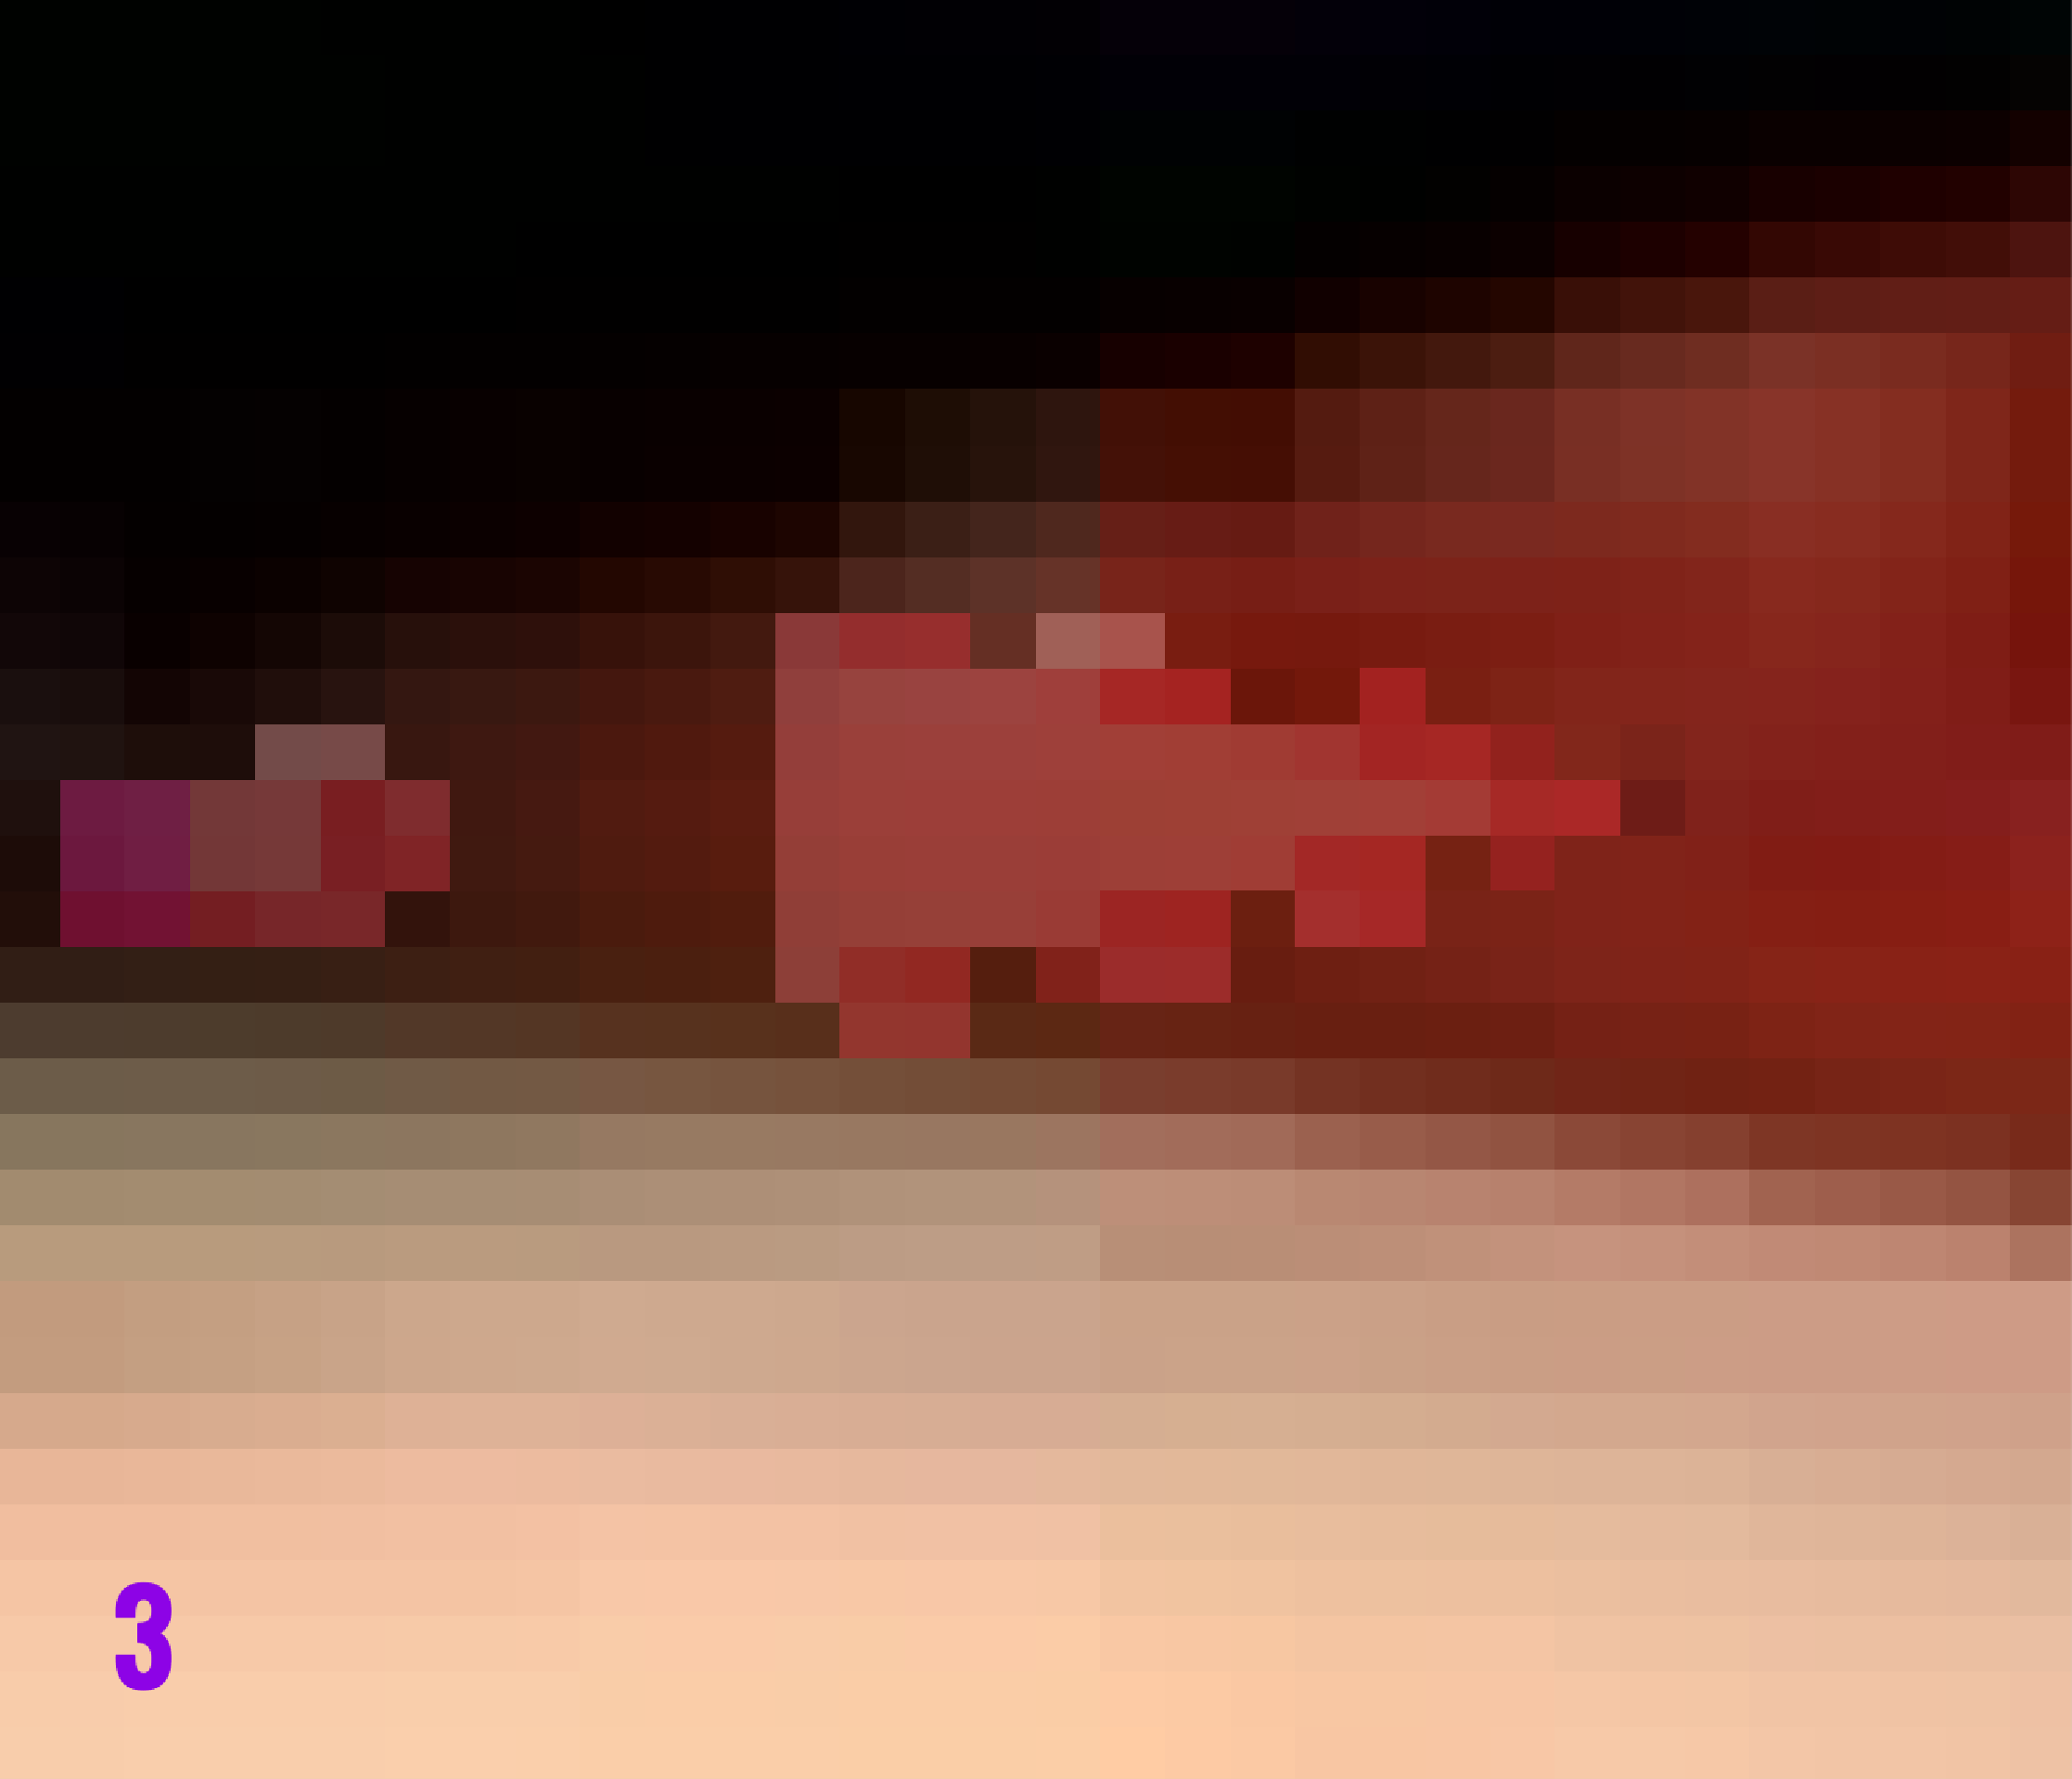
\includegraphics[height=\imgWidth]{images/game_systems/2DumDums.png}
  \caption{Two DumDums standing still because the silent part in their loop is played}
  \label{Beatmover}
  \figsource{own graphic}
\end{figure}


\section{Player interaction}
\subsection{Laser}
The player has a laser that he can shoot to destroy enemies. Ammunition is limited and can be refilled by reaching a checkpoint. If the player attempts to shoot without ammunition a failure sound is played, and a puny particle effect is displayed. If the player hits an enemy, a death sound and -particle-system are played as seen in \cref{DestroyEnemy}.

\begin{figure}[p]
  \centering
  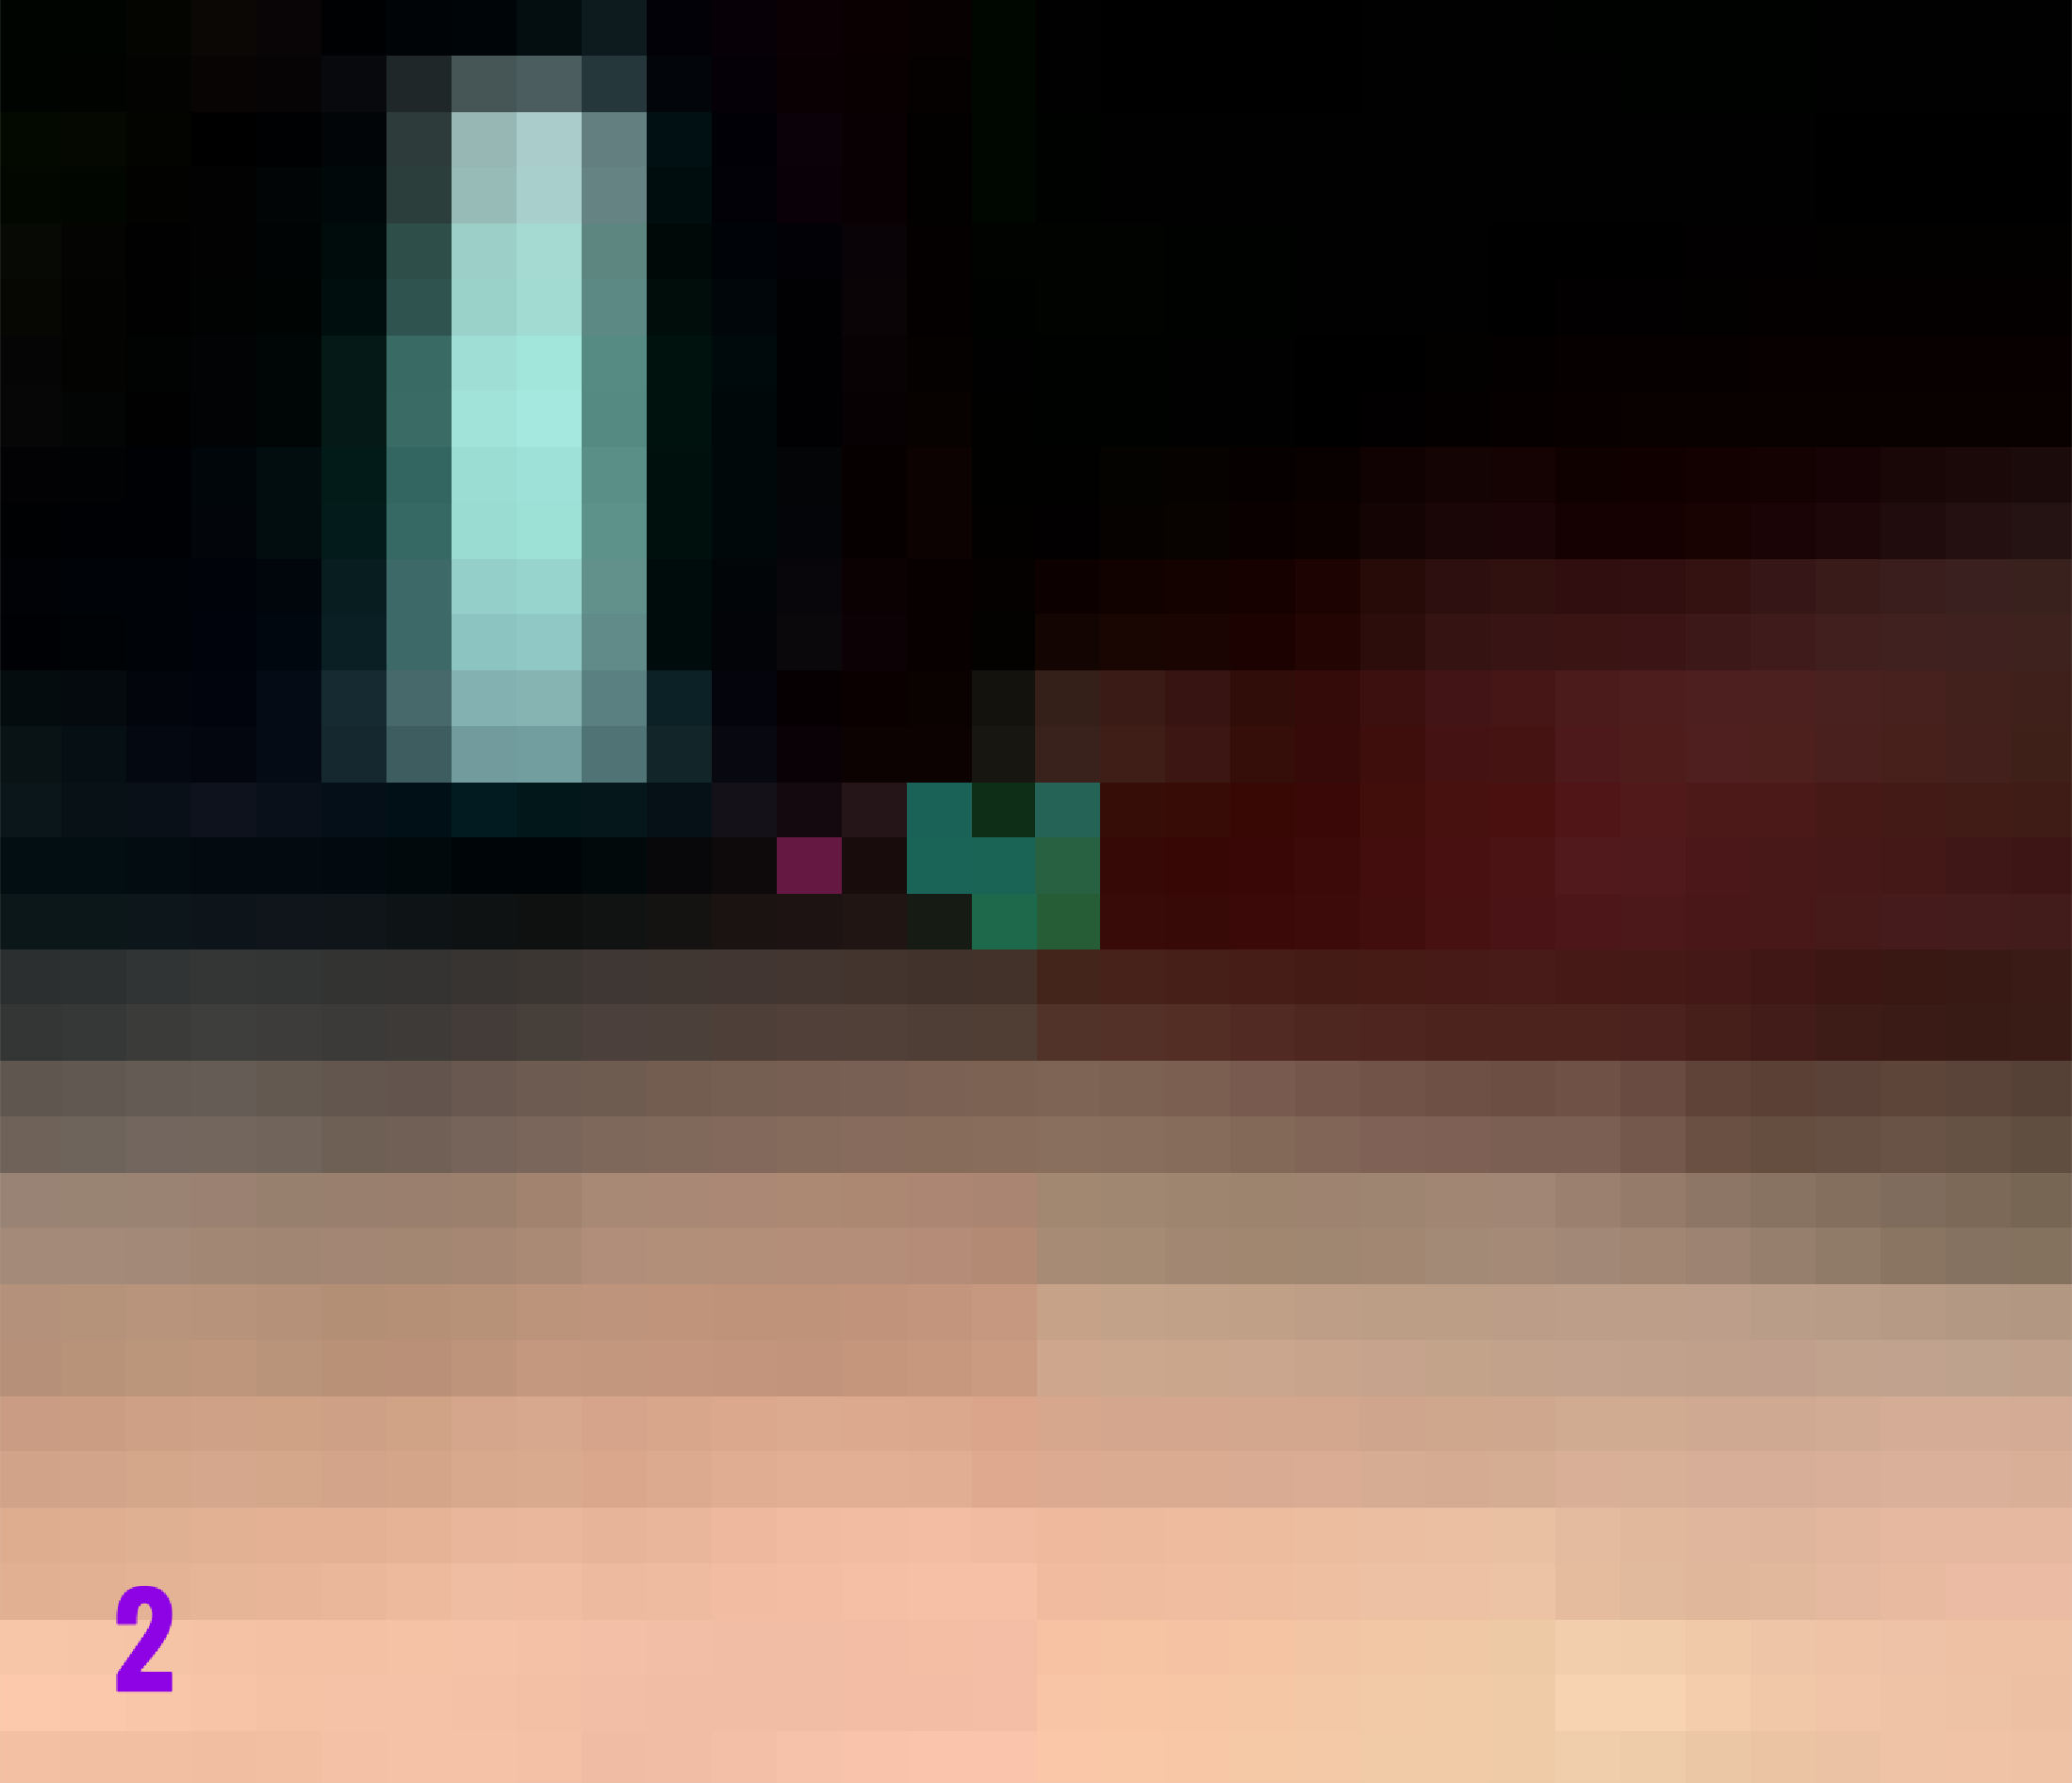
\includegraphics[height=\imgWithTripple, width=\imgWithTripple]{images/game_systems/Shoot1.png} \\[\picVdist]
  \includegraphics[height=\imgWithTripple, width=\imgWithTripple]{images/game_systems/Shoot2.png} \\[\picVdist]
  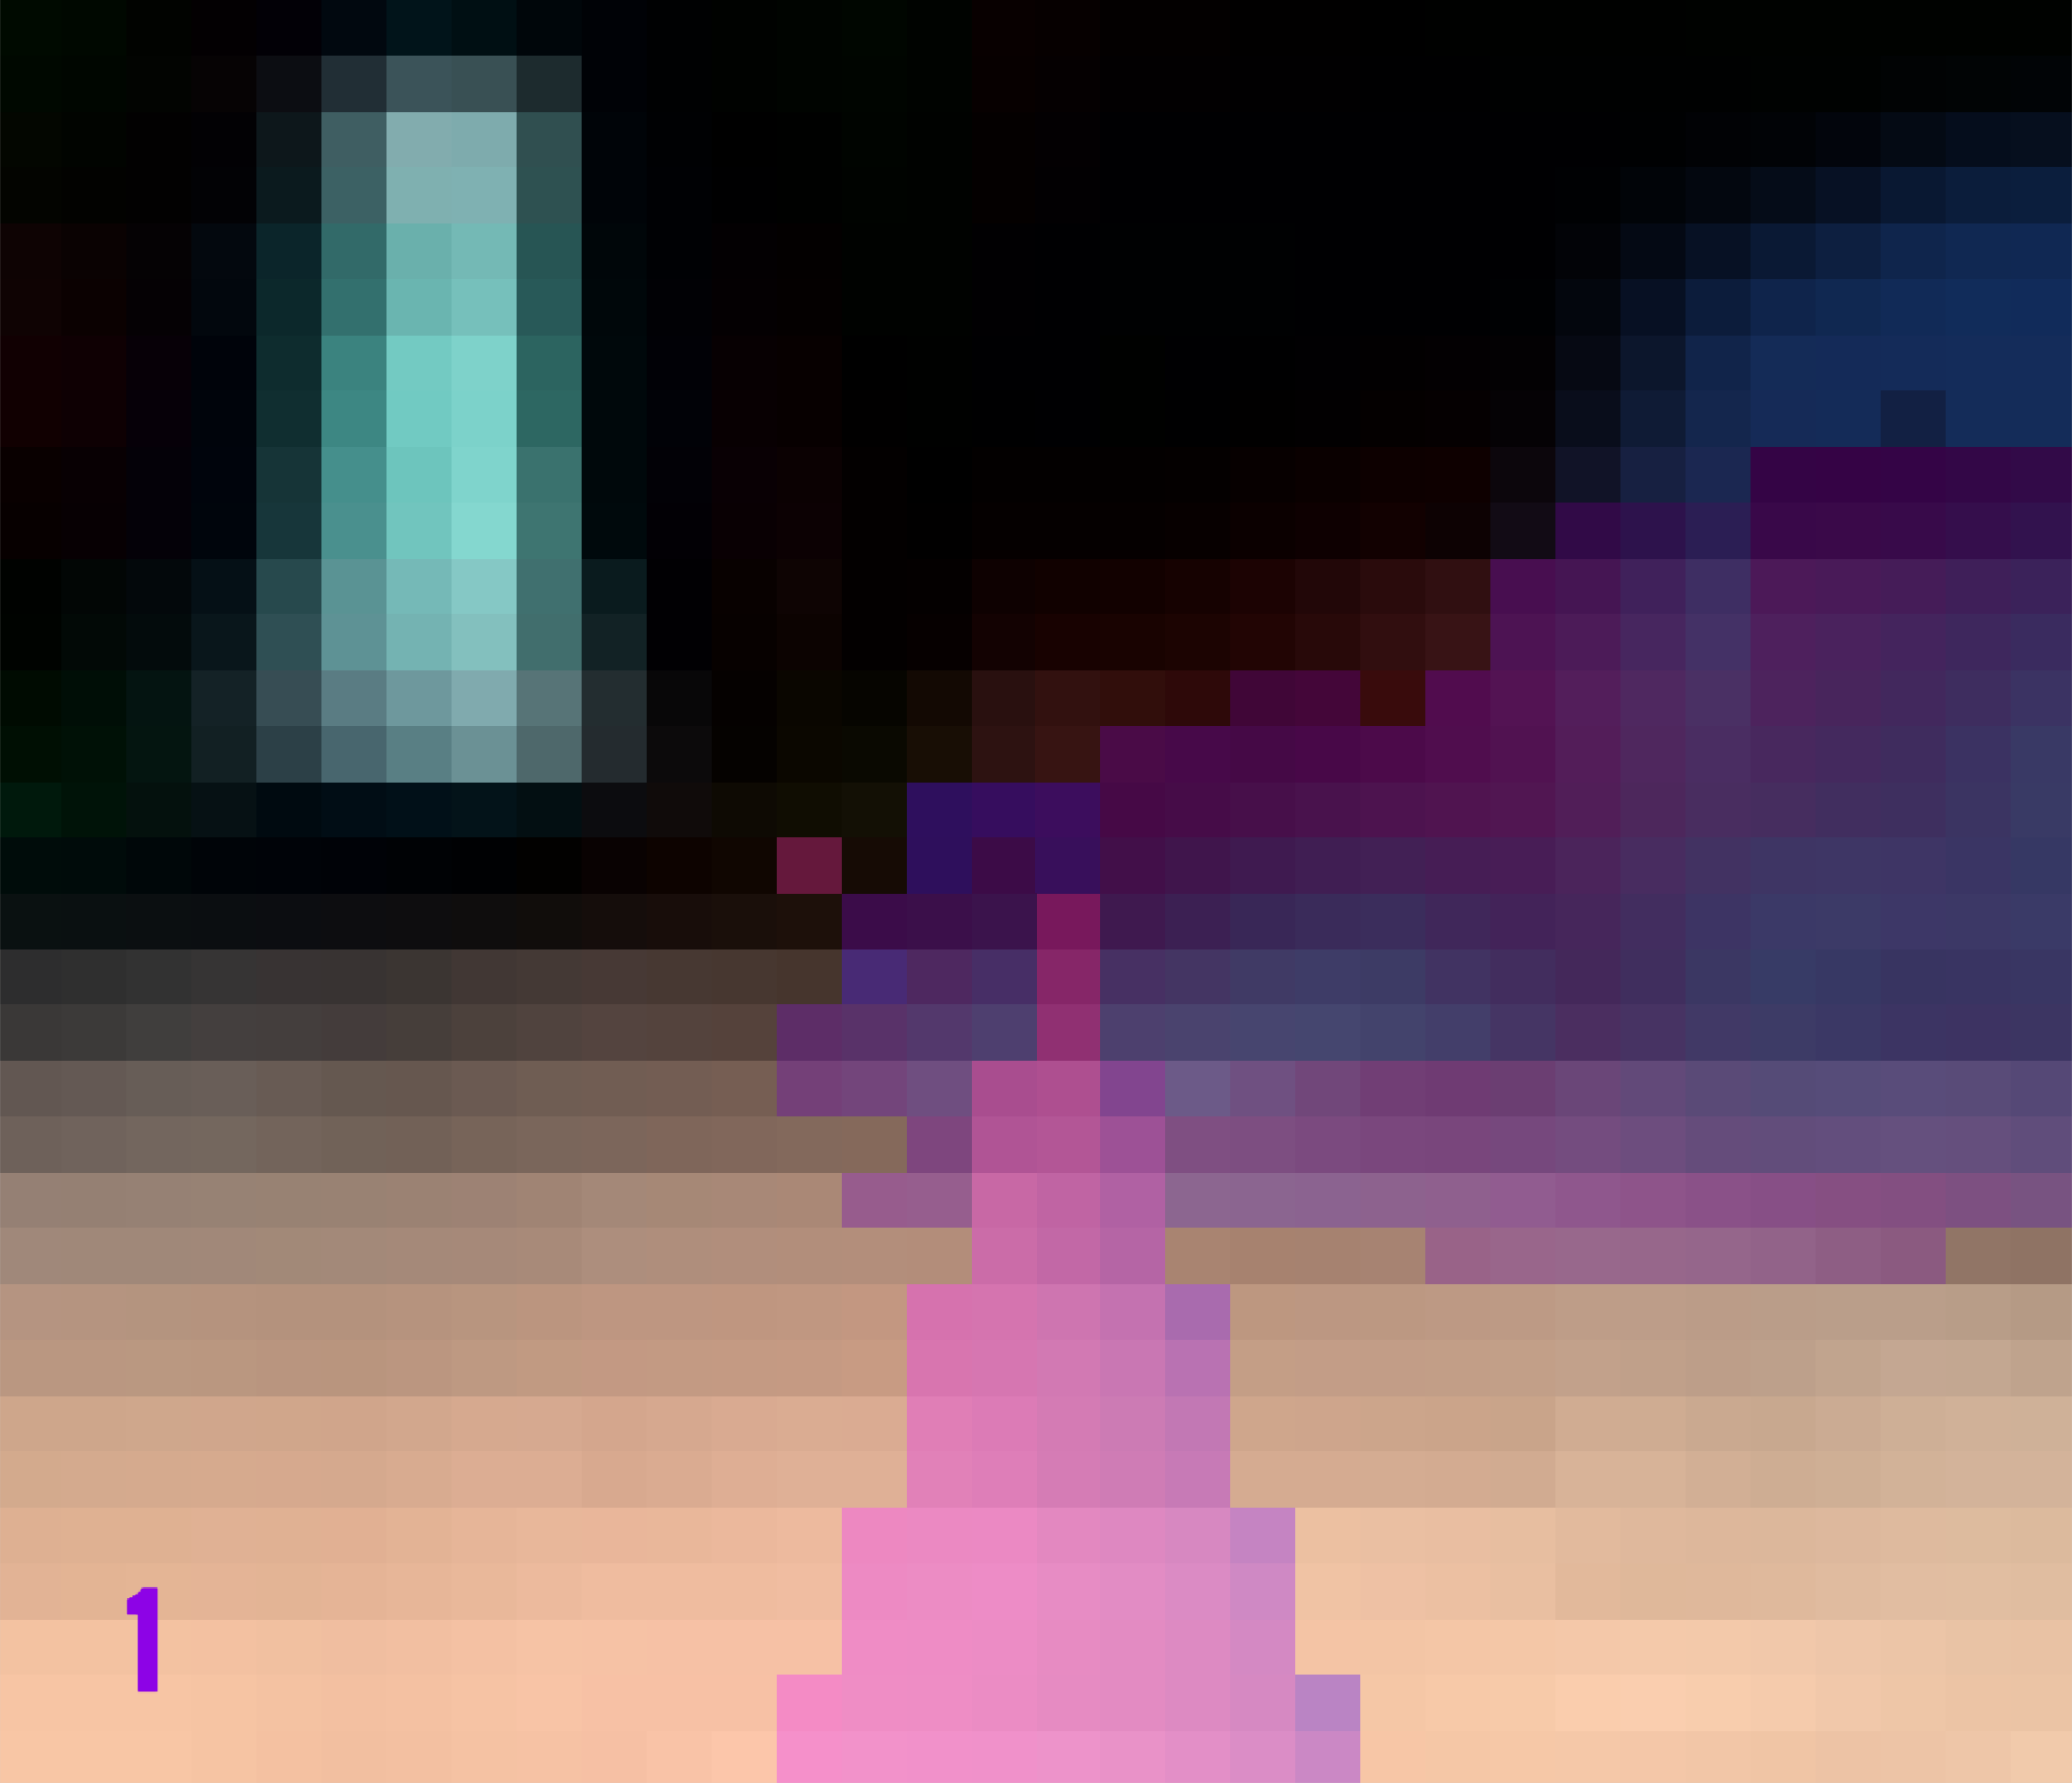
\includegraphics[height=\imgWithTripple, width=\imgWithTripple]{images/game_systems/Shoot3.png}
  \caption{Player destroys an enemy with the laser}
  \label{DestroyEnemy}
  \figsource{own graphic}
\end{figure}


\subsection{Smoke balls}
Smoke emitting  balls can be thrown by the player. As shown in \cref{SmokeInEnvironment}, smoke balls can reveal where hidden structural objects, like walls, are in the Unity environment. Smoke balls can also be used to uncover the invisible champer as seen in \cref{UncoverChamper}. More information on how the smoke ball works can be found in \cref{SmokeBallRendering}.

\begin{figure}[p]
  \centering
  
\includegraphics[width=\imgWidth]{images/game_systems/NoSmoke.png} \\[\picVdist]
  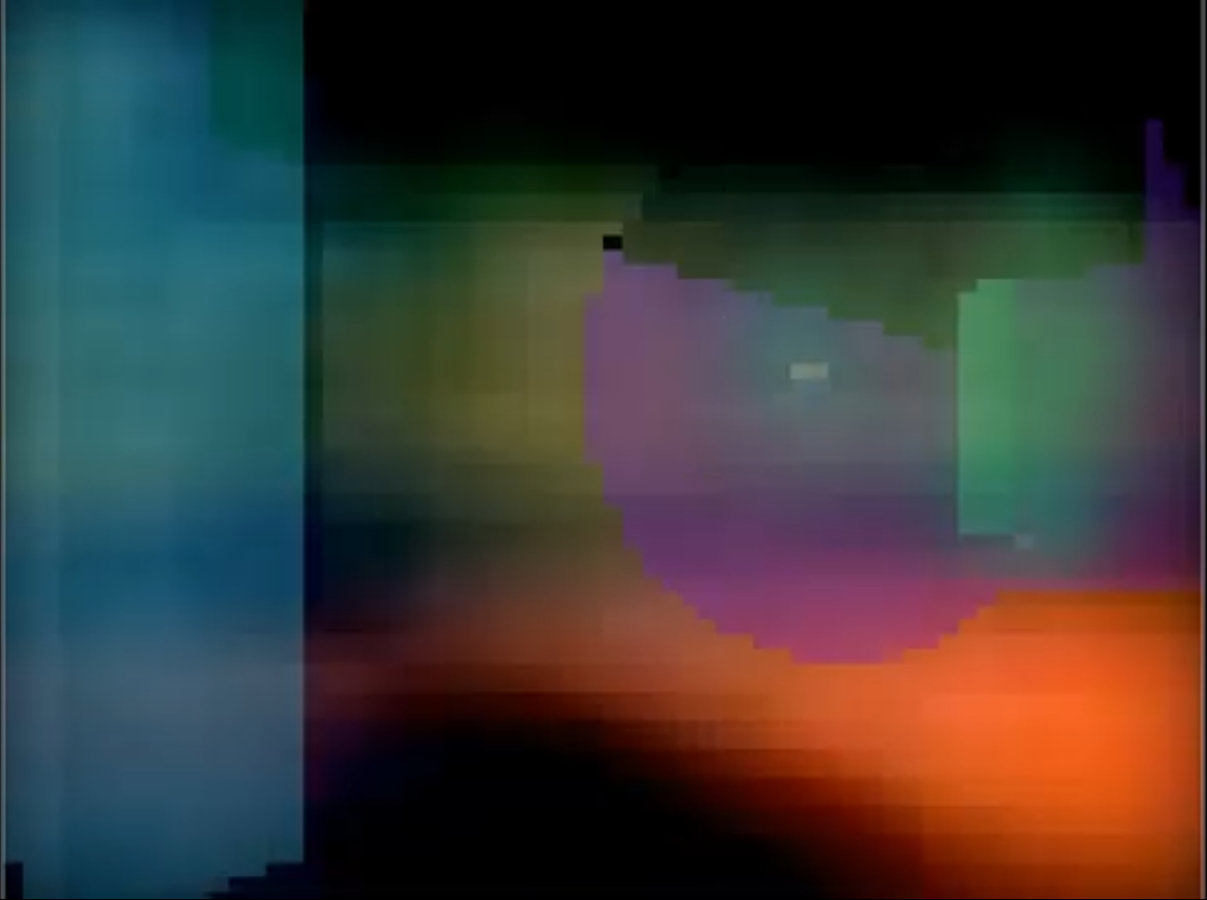
\includegraphics[width=\imgWidth]{images/game_systems/ThrowSmoke.png}
  \caption{Player reveals environment with smoke}
  \label{SmokeInEnvironment}
  \figsource{own graphic}
\end{figure}

\begin{figure}[p]
  \centering
  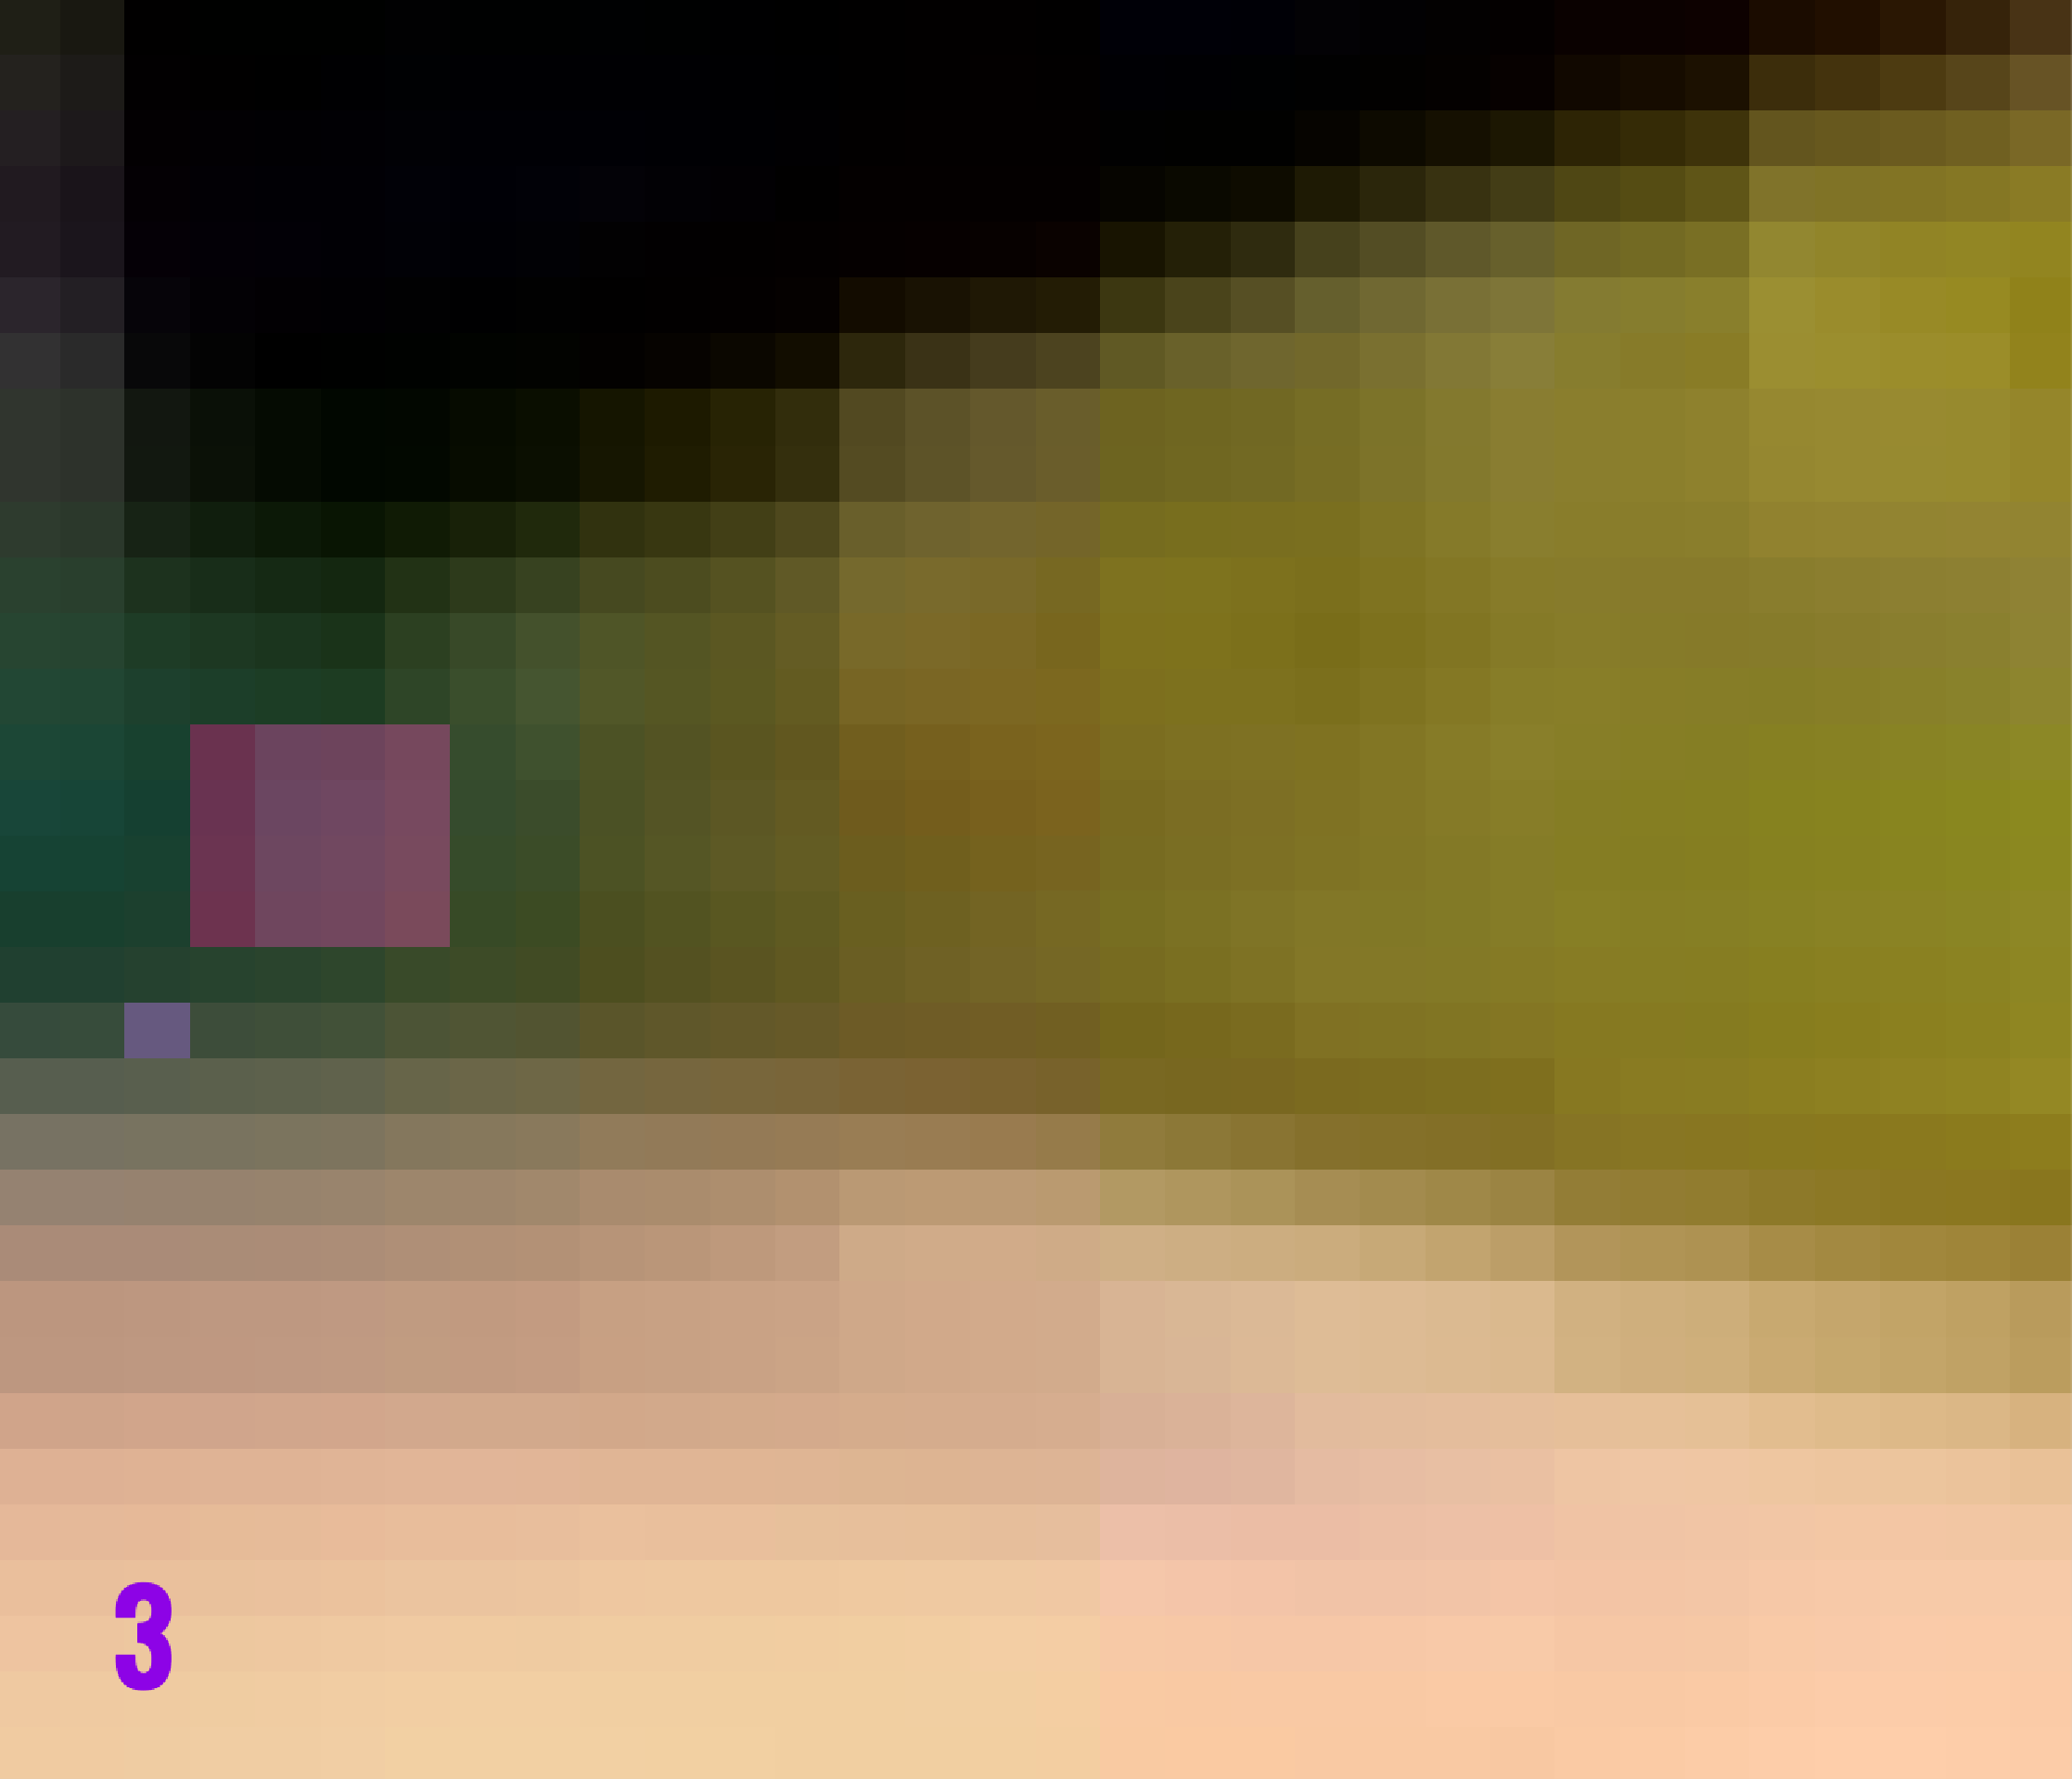
\includegraphics[width=\imgWidth]{images/game_systems/ChamperNoSmoke.png} \\[\picVdist]
  
\includegraphics[width=\imgWidth]{images/game_systems/ChamperInSmoke.png}
  \caption{Player reveals a champer with smoke}
  \label{UncoverChamper}
  \figsource{own graphic}
\end{figure}
